\documentclass[a0paper,portrait]{baposter}

\usepackage{wrapfig}
\usepackage{lmodern}

\usepackage{graphicx} 
\usepackage{subfig}
\usepackage{bm}

\usepackage[utf8]{inputenc} %unicode support
\usepackage[T1]{fontenc}
\usepackage{gensymb} %°


\selectcolormodel{cmyk}

\graphicspath{{figures/}} % Directory in which figures are stored
\renewcommand{\figurename}{Fig.} %rename figure

\newcommand{\compresslist}{%
\setlength{\itemsep}{0pt}%
\setlength{\parskip}{1pt}%
\setlength{\parsep}{0pt}%
}

\newenvironment{boenumerate}
  {\begin{enumerate}\renewcommand\labelenumi{\textbf\theenumi.}}
  {\end{enumerate}}



\begin{document}

\definecolor{PUC}{cmyk}{0.58,0.34,0,0.29}

\begin{poster}
{
grid=false,
headerborder=closed, % Adds a border around the header of content boxes
colspacing=1em, % Column spacing
bgColorOne=white, % Background color for the gradient on the left side of the poster
bgColorTwo=white, % Background color for the gradient on the right side of the poster
borderColor=PUC, % Border color
headerColorOne=PUC, % Background color for the header in the content boxes (left side)
headerColorTwo=PUC, % Background color for the header in the content boxes (right side)
headerFontColor=white, % Text color for the header text in the content boxes
boxColorOne=white, % Background color of the content boxes
textborder=rectangle, %rectangle, % Format of the border around content boxes, can be: none, bars, coils, triangles, rectangle, rounded, roundedsmall, roundedright or faded
eyecatcher=true, % Set to false for ignoring the left logo in the title and move the title left
headerheight=0.135\textheight, % Height of the header
headershape=rectangle, % Specify the rounded corner in the content box headers, can be: rectangle, small-rounded, roundedright, roundedleft or rounded
headershade=plain,
headerfont=\Large\textsf, % Large, bold and sans serif font in the headers of content boxes
%textfont={\setlength{\parindent}{1.5em}}, % Uncomment for paragraph indentation
linewidth=2pt % Width of the border lines around content boxes
}
%
%----------------------------------------------------------------------------------------
%	TITLE AND AUTHOR NAME
%----------------------------------------------------------------------------------------
%
{ %eyecatcher

\includegraphics[scale=0.2]{figures/LogoAndes.jpeg}
}
{ % Poster title
\textsf{Thorium Fuel Cycle in Nuclear Reactors}
}
{% Author names
\sf\vspace{0.5em}
F. Garcia  \& J. Sanabria.\\
\vspace{0.1em}
\small{
Departamento de física, Universidad de los Andes, Bogotá, Colombia. \\
\vspace{0.2em}
fw.garcia@uniandes.edu.co}}


\headerbox{Abstract}{name=Abstract,column=0,row=0, span=3}{
Ferromagnetic and ferroelectric materials undergo phase transitions that allow them to maintain remnant magnetization or electrical polarization at low temperatures, even in the absence of an external field. It has been observed that the introduction of defects in the crystal lattice promotes the appearance of ferroic orders. Recently, a multiferroic transition at room temperature was observed in Te-doped transition metal dichalcogenide $WSe_2$, where the material exhibited the coexistence of ferroelectric and ferromagnetic orders, with a significant influence of vacancies on the emergence of these properties. Based on these studies, it is proposed that similar materials, such as $Mo(Se_{1-x}Te_x)_{2(1-\delta)}$, could exhibit analogous behaviors.\cite{Ferroelectric_MoTe2,Ferromagnetic_MoSe2}
}




\headerbox{1. Introduction}{name=Introduccion,span=1,column=0,below=Abstract}{
Recently, room temperature multiferroicity was observed on the solid solution $W(Se_{1-x}Te_x)_{2(1-\delta)}$ where x represents the Te doping and $\delta$ the chalcogen vacancies, this commposite was formed by the combination of the  semimetal $WSe_2$ and the semiconductor $WTe_2$ \cite{RoomT}. The analysis of multiple stechiometric variations for this solution showed that the doping promoted the formation of vacancies, wich showed to be crucial for the prescence of ferroic orders.
\begin{center}
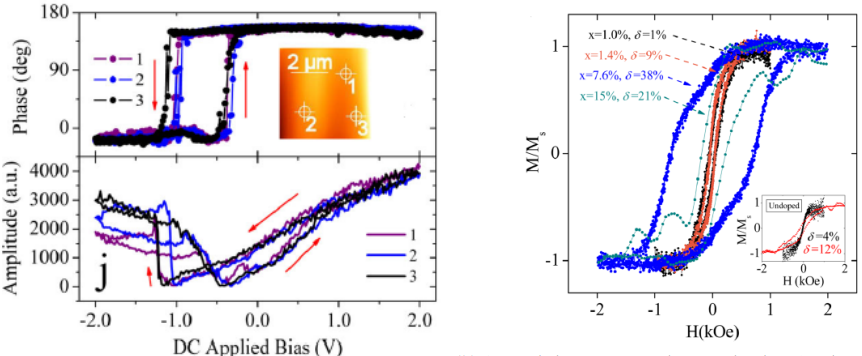
\includegraphics[scale=0.22]{figures/WSe2.png}
\end{center}
\captionof{figure}{\footnotesize PFM and VSM curves for different compositions of $W(Se_{1-x}Te_x)_{2(1-\delta)}$, both curves show the hysteresis characteristic of ferroic orders.}
}


\headerbox{2. Experimental Methods}{name=Metodologia,span=1,column=0,below=Introduccion}{
1. Crystal growth:
\begin{center}
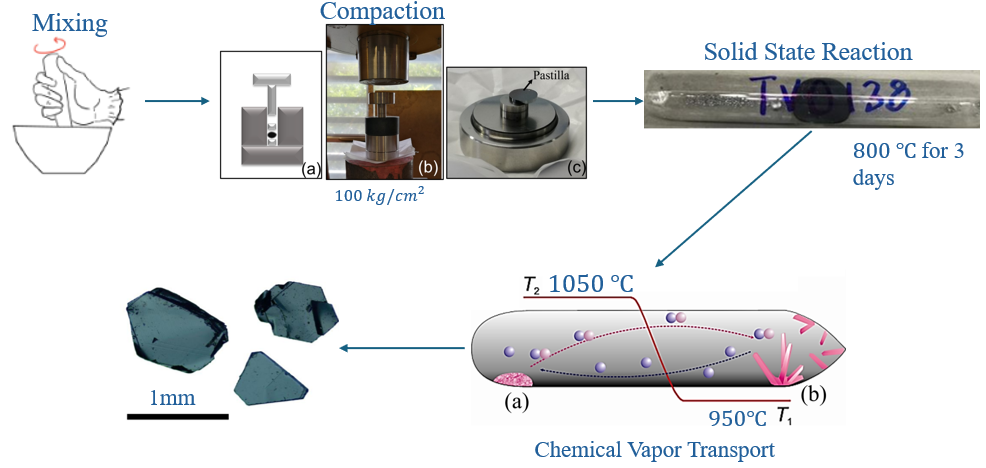
\includegraphics[scale=0.16]{figures/CVY3.png}
\end{center}
\captionof{figure}{\footnotesize Main stages of the growth process for the $Mo(Se_{1-x}Te_x)_{2(1-\delta)}$ crystals.}
2. Techinques used for characterization:
\begin{itemize}
    \item X-Ray Diffraction (XRD) and Raman spectroscopy: To observe changes in the crystal structure due to the introduction of defects.
    \item X-Ray fluorescence: To determine the stoichiometry of different samples.
    \item Vibrating sample magnetometry and piezoelectric force microscopy: To analyze the magnetic and electric orders in different solutions.
\end{itemize}
}


\headerbox{3. Results}{name=Resultados,span=2,column=1,below= Abstract}{
XRD results for multiple compositions of $Mo(Se_{1-x}Te_x)_{2(1-\delta)}$ show that the main diffraction peaks correspond to the (00l) family of planes, which display a shift in the $2\theta$ angle where the peaks are located. Since these planes are directly related to the lattice parameter \textit{c}, the shift represents a variation in the magnitude of \textit{c}. In the second figure, it can be observed that the lattice parameter \textit{c} increases with the amount of doping in the samples.
\begin{center}
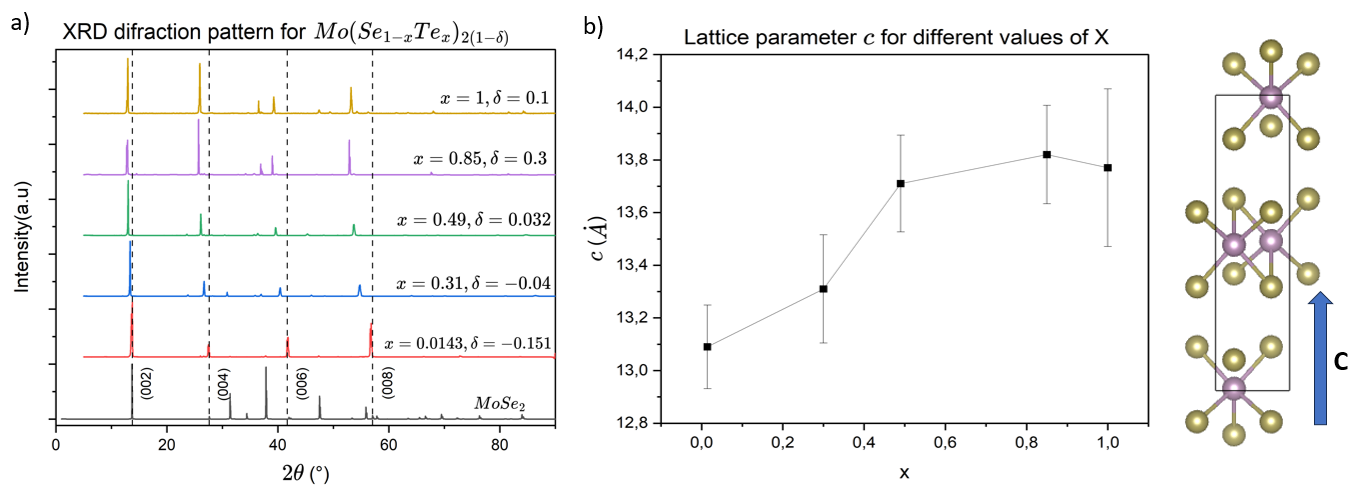
\includegraphics[scale=0.3]{figures/XRDFfinal.png}
\end{center}
\captionof{figure}{\footnotesize a) shows the XRD pattern for multiple solutions of $Mo(Se_{1-x}Te_x)_{2(1-\delta)}$ compared to the expected peaks for $MoSe_2$. b) shows the calculated values for the lattice parameter \textit{c}, based on the observed diffraction pattern. }
The Raman spectra for multiple compositions of $Mo(Se_{1-x}Te_x)_{2(1-\delta)}$ show that the dominant phase in the solutions varies depending on the doping level. It was observed that this dominant phase corresponds to the pure composition closest to the one under analysis. Furthermore, for compositions closer to $MoTe_2$, peaks associated with both the 2H and 1T' crystal phases were observed, indicating a coexistence of crystal phases, with the 1T' phase being dominant.

\begin{center}
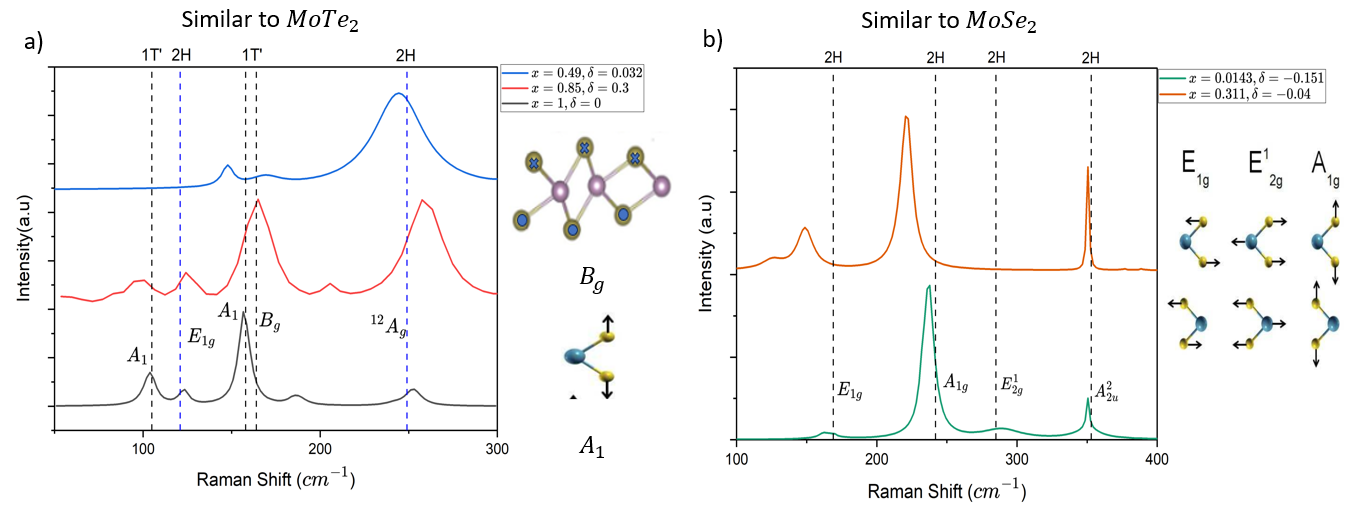
\includegraphics[scale=0.31]{figures/RamanFinalll.png}
\end{center}
\captionof{figure}{\footnotesize The Raman spectra for multiple compositions of $Mo(Se_{1-x}Te_x)_{2(1-\delta)}$ show that the dominant phase in the solutions changes with the doping level. Figure (a) presents the Raman spectrum that most closely resembles that of pure $MoTe_2$ compared to the expected peaks (vertical lines), along with a representation of the $B_g$ and $A_1$ Raman modes. It can be observed that some peaks correspond to different crystal phases. Figure (b) presents the Raman spectrum that most closely resembles $MoSe_2$ in its 2H crystal phase compared to the expected peaks (vertical lines), along with a representation of the $A_{1g}$ and $E_g$ Raman modes.}

Both sets of results indicate that the introduction of crystal defects significantly alters the crystal structure, changing the dominant crystal phase. This causes effects such as an increase in lattice parameters and the breaking of centrosymmetry due to the transition to the 1T' phase.
}
\headerbox{4.Conclusions and future work}{name=Conclusiones,column=1,below=Resultados,span=2}{The crystallographic analysis shows that doping effectively distorts the crystal structure, altering both the lattice parameters and the crystal phase, indicating a breaking of centrosymmetry in the system. This symmetry breaking is identified as a factor inducing spontaneous polarization in crystal systems. Future work should focus on identifying the direct effect of vacancies on the crystal structure by producing compositions with more controlled vacancies. In parallel with crystal structure analysis, the effects of both doping and vacancies on the ferroic orders of the solution remain to be analyzed.
}

\headerbox{ References}{name=Referecencias,column=0,below=Metodologia,span=1}{

\footnotesize 
\renewcommand{\section}[2]{\vskip 0.05em} % Get rid of the default "References" section title
\nocite{*} % Insert publications even if they are not cited in the poster

\bibliographystyle{naturemag}
\bibliography{poster} % Use sample.bib as the bibliography file
}

\end{poster}

\end{document}